% !TEX program = xelatex
\documentclass[11pt, a4paper]{article}

% ====== Packages ======
\usepackage[margin=2.5cm]{geometry}
\usepackage{amsmath, amssymb, amsthm}
\usepackage{graphicx}
\usepackage{booktabs}
\usepackage[hidelinks]{hyperref}
\usepackage{algorithm}
\usepackage{algpseudocode}
\usepackage{xcolor}
\usepackage{enumitem}
\usepackage{float}
\usepackage{subcaption}
\usepackage{tikz}
\usetikzlibrary{arrows.meta, positioning, shapes.geometric, fit}

% ====== Theorems ======
\newtheorem{definition}{Definition}
\newtheorem{theorem}{Theorem}
\newtheorem{proposition}{Proposition}
\newtheorem{lemma}{Lemma}

% ====== Title ======
\title{\textbf{Ouroboros V22: Bayesian Scenario Simulation and\\Recurrent Depth Cognition for Autonomous\\Financial Decision-Making}}

\author{
  Mian Zhang\\
  Independent Researcher\\
  Ouroboros Project\\
  \texttt{373743743@qq.com}
}

\date{April 2026}

\begin{document}
\maketitle

% ====== Abstract ======
\begin{abstract}
We present Ouroboros V22, a cognitive architecture for autonomous financial decision-making that integrates three novel components: (1) a \textbf{Bayesian Scenario Simulation Engine} that generates regime-aware posterior probability distributions over market scenarios and computes expected value across actions; (2) a \textbf{Recurrent Depth Cognitive Engine (RDCE)} inspired by the OpenMythos architecture, which applies iterative refinement through Linear Time-Invariant (LTI) injection and Adaptive Computation Time (ACT) halting; and (3) a \textbf{6-Layer Unified Memory System} with Hawkes-process temporal decay that enables closed-loop calibration between decisions and outcomes. The system operates a 16-node parallel inference swarm where specialized agents debate across market domains (crypto, equities, forex, commodities, derivatives), with their outputs fused through a hierarchical Wave-1/2/3 architecture. We demonstrate the integration through a 5-hook pipeline that connects signal ingestion, scenario simulation, multi-agent debate, supreme decision, and post-decision memory calibration into a self-evolving cognitive loop. Preliminary distillation experiments using Claude as teacher model show that V22-enhanced prompts (with scenario context and causal chain injection) produce training data with 0.79 mean quality score across 8 financial market categories.
\end{abstract}

\section{Introduction}

Autonomous financial decision-making in non-stationary markets remains an open challenge. While Large Language Models (LLMs) have shown impressive reasoning capabilities \cite{openai2023gpt4, dubey2024llama3}, their application to high-stakes sequential decision-making under regime uncertainty requires three capabilities that standard LLM architectures lack:

\begin{enumerate}[leftmargin=*]
  \item \textbf{Scenario Imagination}: The ability to simulate multiple future trajectories with calibrated probability estimates, conditioned on the current market regime.
  \item \textbf{Adaptive Depth}: The ability to allocate more computation to complex or ambiguous situations (crisis vs. range-bound markets).
  \item \textbf{Self-Calibrating Memory}: The ability to update internal priors based on the outcomes of past decisions, creating a closed-loop learning system.
\end{enumerate}

This paper describes Ouroboros V22, a cognitive architecture that addresses all three gaps through the introduction of a Bayesian Scenario Simulation Engine (\S\ref{sec:bayesian}), a Recurrent Depth Cognitive Engine (\S\ref{sec:rdce}), and a 6-Layer Unified Memory System (\S\ref{sec:memory}). These components are integrated into a live 16-node swarm inference pipeline through a 5-hook architecture (\S\ref{sec:integration}).

\subsection{Relation to Prior Work in This Series}

This is the fourth paper in the Reflexive Intelligence research program:
\begin{itemize}[leftmargin=*]
  \item \textbf{Paper 1} \cite{paper1}: Established the theoretical framework for Observer-Participant Environments (OPE) and reflexive decision-making.
  \item \textbf{Paper 2} \cite{paper2}: Introduced ReflexBench, demonstrating that reflexive reasoning emerges as a phase transition during GRPO training.
  \item \textbf{Paper 3} \cite{paper3}: Analyzed structural interference in multi-objective reward functions and the topology of reward interaction.
  \item \textbf{This paper (Paper 4)}: Operationalizes these theoretical insights into a production cognitive architecture.
\end{itemize}


% ============================================================
\section{Bayesian Scenario Simulation Engine}
\label{sec:bayesian}
% ============================================================

\subsection{Motivation}

In financial markets, the key cognitive challenge is not prediction but \emph{scenario imagination}: ``What are the plausible futures, and what is the expected value of each action under each scenario?'' We formalize this as a Bayesian inference problem conditioned on market regime.

\subsection{Formal Framework}

\begin{definition}[Market Regime]
Let $\mathcal{R} = \{r_1, \ldots, r_K\}$ be the set of market regimes (e.g., CRISIS, BULLISH, BEARISH, HIGH\_VOL, RANGE, ARMAGEDDON). The current regime $r_t$ is estimated from observable signals via a Hidden Markov Model.
\end{definition}

\begin{definition}[Scenario Space]
Given regime $r_t$ and event context $e_t$, we define the scenario space as $\mathcal{S} = \{s_1, \ldots, s_N\}$ where each scenario $s_i$ represents a plausible future market trajectory over horizon $\tau$.
\end{definition}

The engine generates scenarios via a $3 \times 3$ template matrix:
\begin{equation}
  \mathcal{S} = \{(\text{direction}, \text{horizon})\} = \{\text{bull}, \text{base}, \text{bear}\} \times \{\text{short}, \text{mid}, \text{long}\}
\end{equation}

\subsubsection{Prior Distribution}

The prior probability of each scenario is conditioned on the current regime:
\begin{equation}
  P(s_i | r_t) = \text{REGIME\_PRIORS}[r_t][s_i]
\end{equation}

For example, in CRISIS regime:
\begin{equation}
  P(\text{bear}|\text{CRISIS}) = 0.50, \quad P(\text{base}|\text{CRISIS}) = 0.30, \quad P(\text{bull}|\text{CRISIS}) = 0.20
\end{equation}

\subsubsection{Likelihood from Swarm Intelligence}

Given the Wave-1 responses $\{w_1, \ldots, w_M\}$ from $M$ specialized nodes, we compute a sentiment likelihood:
\begin{equation}
  P(w_{1:M} | s_i) \propto \exp\left(\beta \cdot \text{sentiment\_alignment}(w_{1:M}, s_i)\right)
\end{equation}

where $\text{sentiment\_alignment}$ measures the cosine similarity between the aggregate node sentiment and each scenario's directional hypothesis.

\subsubsection{Posterior and Expected Value}

The posterior is computed via Bayes' rule:
\begin{equation}
  P(s_i | r_t, w_{1:M}) = \frac{P(w_{1:M} | s_i) \cdot P(s_i | r_t)}{\sum_j P(w_{1:M} | s_j) \cdot P(s_j | r_t)}
\end{equation}

The expected value of action $a \in \{\text{LONG}, \text{SHORT}, \text{NEUTRAL}\}$ is:
\begin{equation}
  \text{EV}(a) = \sum_{i=1}^{N} P(s_i | r_t, w_{1:M}) \cdot R(a, s_i)
\end{equation}

where $R(a, s_i)$ is the payoff matrix:
\begin{equation}
R(a, s_i) = \begin{cases}
  +\alpha_{\text{bull}} & \text{if } a=\text{LONG}, s_i \in \text{bull scenarios} \\
  -\delta_{\text{bull}} & \text{if } a=\text{SHORT}, s_i \in \text{bull scenarios} \\
  0 & \text{if } a=\text{NEUTRAL}
\end{cases}
\end{equation}

\subsubsection{Divergence Detection}

We compute the KL divergence between the swarm-updated posterior and the regime prior:
\begin{equation}
  D_{\text{KL}}(P_{\text{post}} \| P_{\text{prior}}) = \sum_i P_{\text{post}}(s_i) \log \frac{P_{\text{post}}(s_i)}{P_{\text{prior}}(s_i)}
\end{equation}

High divergence ($D_{\text{KL}} > 0.8$) triggers a ``Caution'' flag that instructs the Supreme model to reduce leverage and increase hedge ratios.


% ============================================================
\section{Recurrent Depth Cognitive Engine (RDCE)}
\label{sec:rdce}
% ============================================================

\subsection{Motivation}

Standard transformer inference processes input in a single forward pass, allocating identical computation regardless of problem complexity. Financial decision-making exhibits widely varying complexity: a range-bound market requires minimal analysis, while a regime transition event demands deep multi-factor reasoning.

We address this through a Recurrent Depth mechanism inspired by OpenMythos \cite{openmythos}, where a subset of transformer layers is executed iteratively, with each loop corresponding to a distinct cognitive stage.

\subsection{Architecture}

Given a base model (Qwen3.5-35B) with layers $\{L_1, \ldots, L_{64}\}$, we designate layers $L_8$ through $L_{15}$ as the \textbf{recurrent block} $\mathcal{B}$. For $K$ recurrent loops:

\begin{equation}
  h^{(k+1)} = \mathcal{B}(h^{(k)}) + A \cdot h^{(k)} + B \cdot e^{(k)}
\end{equation}

where:
\begin{itemize}
  \item $h^{(k)}$ is the hidden state at loop $k$
  \item $A \in \mathbb{R}^{d \times d}$ is the LTI state transition matrix with $\rho(A) < 1$ (spectral radius constraint for stability)
  \item $B \in \mathbb{R}^{d \times d_e}$ is the input injection matrix
  \item $e^{(k)}$ is the loop index embedding (encoding which cognitive stage the model is in)
\end{itemize}

\subsection{Cognitive Stage Mapping}

Each loop is assigned a cognitive stage through the loop index embedding:

\begin{table}[H]
\centering
\begin{tabular}{clc}
\toprule
\textbf{Loop Range} & \textbf{Cognitive Stage} & \textbf{Function} \\
\midrule
1--5 & Perception & Signal identification and anomaly detection \\
6--10 & Mechanism & Transmission channel analysis \\
11--15 & Causal & Causal chain reasoning \\
16--20 & Reflexive & Self-questioning and blind spot detection \\
21--30 & Synthesis & Decision integration and kill-switch definition \\
\bottomrule
\end{tabular}
\caption{Mapping from recurrent depth loops to cognitive stages.}
\label{tab:cognitive_stages}
\end{table}

\subsection{Adaptive Computation Time (ACT)}

The number of loops $K$ is determined dynamically based on market complexity:

\begin{equation}
  \text{complexity} = w_v \cdot \sigma_{20d} + w_r \cdot \mathbb{1}[\text{regime} \in \{\text{CRISIS}, \text{ARMAGEDDON}\}] + w_c \cdot \mathbb{1}[\text{signal\_conflict}]
\end{equation}

\begin{equation}
  K = K_{\min} + \lfloor (K_{\max} - K_{\min}) \cdot \text{complexity} \rfloor
\end{equation}

where $K_{\min} = 5$, $K_{\max} = 30$, $w_v = 0.4$, $w_r = 0.4$, $w_c = 0.3$. A halting mechanism monitors the cosine similarity between consecutive hidden states:

\begin{equation}
  \text{halt if } \cos(h^{(k)}, h^{(k-1)}) > \theta_{\text{halt}} = 0.98
\end{equation}

\subsection{Parameter Efficiency}

The RDCE adds only $\sim$5M trainable parameters to the frozen 35B base:
\begin{itemize}
  \item LTI matrices $A, B$: $\sim$2M parameters
  \item Per-loop LoRA adapters (rank=4): $\sim$2M parameters
  \item Loop index embeddings: $\sim$0.5M parameters
  \item ACT halting head: $\sim$0.5M parameters
\end{itemize}


% ============================================================
\section{6-Layer Unified Memory System}
\label{sec:memory}
% ============================================================

\subsection{Architecture}

The memory system consists of six layers with distinct temporal characteristics:

\begin{table}[H]
\centering
\begin{tabular}{clll}
\toprule
\textbf{Layer} & \textbf{Name} & \textbf{Content} & \textbf{Decay} \\
\midrule
L1 & Regime Memory & Per-node $\times$ per-regime win/loss records & Hawkes $\lambda=0.95$ \\
L2 & Signal Cache & Raw signal snapshots & Rolling window (24h) \\
L3 & Forum Memory & Debate precedents and outcomes & Hawkes $\lambda=0.90$ \\
L4 & Decision Trail & Full decision audit trail & Persistent (no decay) \\
L5 & Causal KG & Knowledge graph of causal chains & Lazy-loaded, persistent \\
L6 & Semantic Store & Vector embeddings of past reasoning & Cosine retrieval \\
\bottomrule
\end{tabular}
\caption{6-Layer Unified Memory Architecture.}
\label{tab:memory}
\end{table}

\subsection{Hawkes Process Temporal Decay}

For layers L1 and L3, memory relevance decays via a Hawkes self-exciting process:

\begin{equation}
  \lambda(t) = \mu + \sum_{t_i < t} \alpha \cdot e^{-\beta(t - t_i)}
\end{equation}

where $\mu$ is the base relevance, $\alpha$ controls self-excitation (a correct prediction boosts nearby memories), and $\beta$ controls decay rate. This prevents ``dogmatic memory''—the system naturally forgets stale regime patterns while reinforcing recently validated ones.

\subsection{Closed-Loop Calibration}

After each decision epoch, the post-decision hook updates all memory layers:

\begin{algorithm}[H]
\caption{Post-Decision Memory Calibration}
\begin{algorithmic}[1]
\Require Decision $d_t$, PnL outcome $\pi_t$, regime $r_t$
\State \textbf{L1:} Update regime memory: $\text{win\_rate}[r_t] \leftarrow \text{EMA}(\mathbb{1}[\pi_t > 0])$
\State \textbf{L3:} Store debate precedent with outcome label
\State \textbf{L4:} Append full decision record to audit trail
\State \textbf{L6:} Store reasoning embedding for future retrieval
\State \textbf{Bayesian:} Calibrate scenario prior:
\State \quad $P_{\text{new}}(s_i | r_t) \leftarrow \alpha \cdot P_{\text{old}}(s_i | r_t) + (1-\alpha) \cdot \mathbb{1}[s_i = s_{\text{realized}}]$
\end{algorithmic}
\end{algorithm}


% ============================================================
\section{5-Hook Integration Architecture}
\label{sec:integration}
% ============================================================

The three subsystems are connected to the Ouroboros swarm engine through 5 integration hooks:

\begin{figure}[H]
\centering
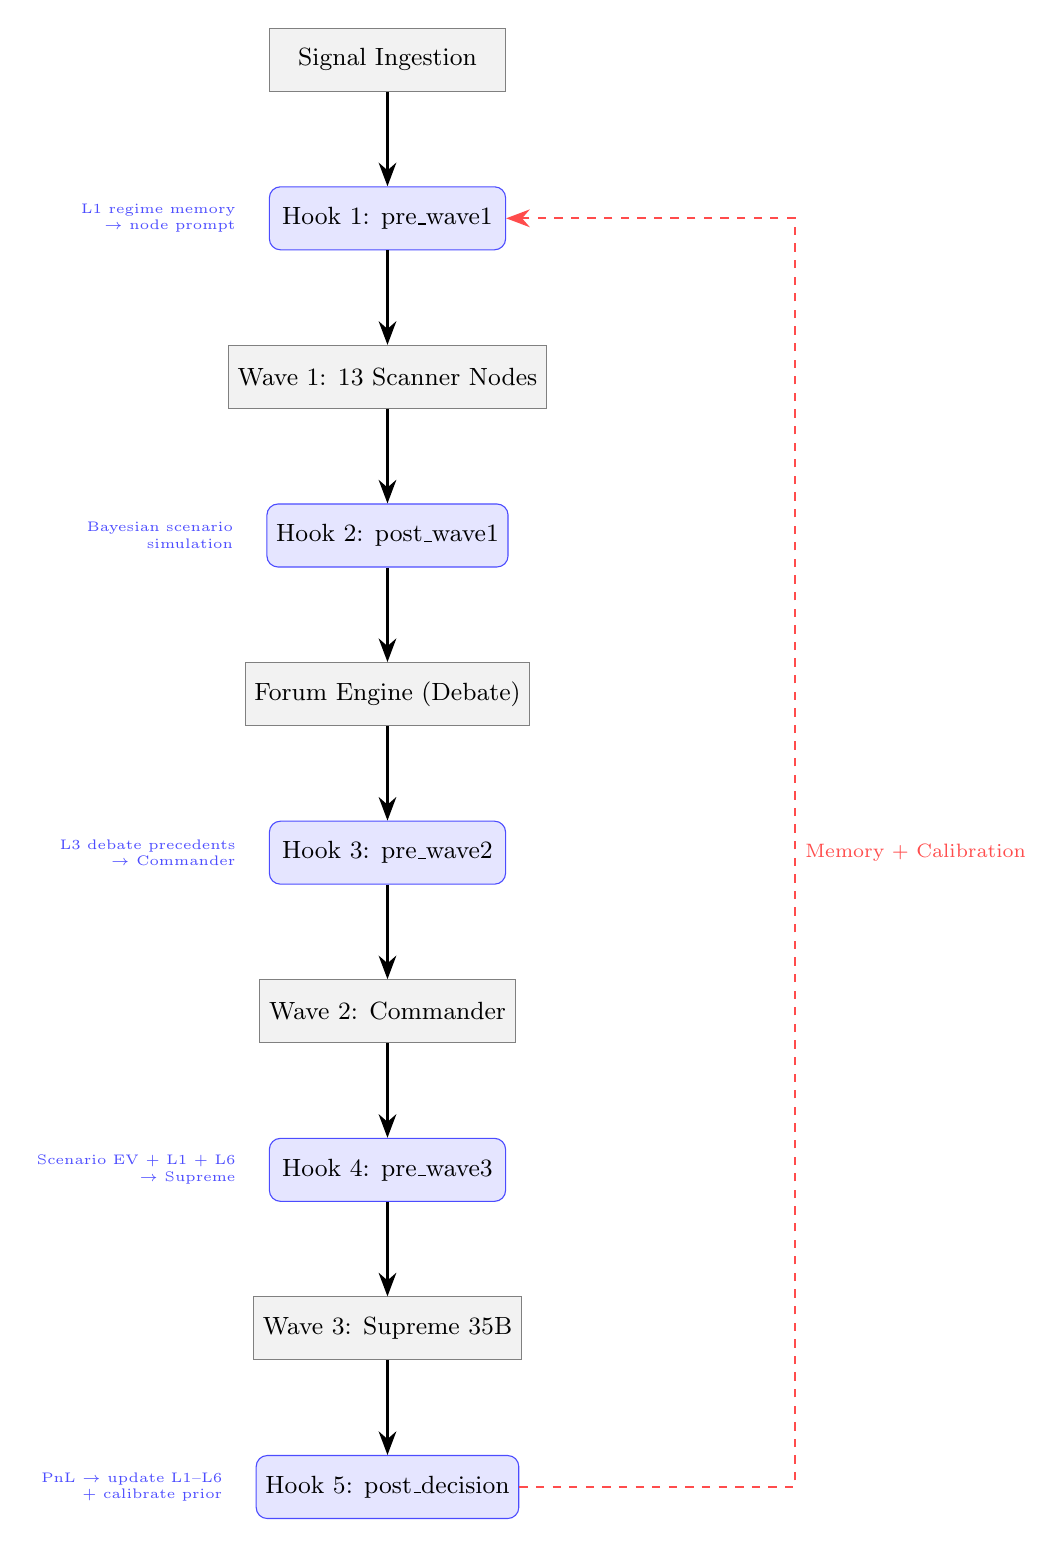
\begin{tikzpicture}[
  node distance=1.2cm,
  hook/.style={rectangle, rounded corners, draw=blue!70, fill=blue!10, minimum width=3cm, minimum height=0.8cm, font=\small},
  stage/.style={rectangle, draw=black!50, fill=gray!10, minimum width=3cm, minimum height=0.8cm, font=\small},
  arr/.style={-{Stealth[length=3mm]}, thick}
]
  \node[stage] (s1) {Signal Ingestion};
  \node[hook, below=of s1] (h1) {Hook 1: pre\_wave1};
  \node[stage, below=of h1] (s2) {Wave 1: 13 Scanner Nodes};
  \node[hook, below=of s2] (h2) {Hook 2: post\_wave1};
  \node[stage, below=of h2] (s3) {Forum Engine (Debate)};
  \node[hook, below=of s3] (h3) {Hook 3: pre\_wave2};
  \node[stage, below=of h3] (s4) {Wave 2: Commander};
  \node[hook, below=of s4] (h4) {Hook 4: pre\_wave3};
  \node[stage, below=of h4] (s5) {Wave 3: Supreme 35B};
  \node[hook, below=of s5] (h5) {Hook 5: post\_decision};

  \draw[arr] (s1) -- (h1);
  \draw[arr] (h1) -- (s2);
  \draw[arr] (s2) -- (h2);
  \draw[arr] (h2) -- (s3);
  \draw[arr] (s3) -- (h3);
  \draw[arr] (h3) -- (s4);
  \draw[arr] (s4) -- (h4);
  \draw[arr] (h4) -- (s5);
  \draw[arr] (s5) -- (h5);

  % memory feedback
  \draw[arr, dashed, red!70] (h5.east) -- ++(3.5,0) |- node[right, pos=0.25, font=\scriptsize, text=red!70] {Memory + Calibration} (h1.east);

  % annotations (left side to avoid feedback line)
  \node[left=0.3cm of h1, font=\tiny, text=blue!70, align=right] {L1 regime memory\\$\rightarrow$ node prompt};
  \node[left=0.3cm of h2, font=\tiny, text=blue!70, align=right] {Bayesian scenario\\simulation};
  \node[left=0.3cm of h3, font=\tiny, text=blue!70, align=right] {L3 debate precedents\\$\rightarrow$ Commander};
  \node[left=0.3cm of h4, font=\tiny, text=blue!70, align=right] {Scenario EV + L1 + L6\\$\rightarrow$ Supreme};
  \node[left=0.3cm of h5, font=\tiny, text=blue!70, align=right] {PnL $\rightarrow$ update L1--L6\\+ calibrate prior};
\end{tikzpicture}
\caption{5-Hook integration architecture connecting the Bayesian engine, RDCE, and memory system to the Ouroboros swarm pipeline.}
\label{fig:hooks}
\end{figure}

\begin{enumerate}[leftmargin=*]
  \item \textbf{Hook 1 (pre\_wave1)}: Injects L1 (regime-specific) and L5 (causal KG) memories into each scanner node's system prompt. Nodes receive historical context relevant to their domain.
  \item \textbf{Hook 2 (post\_wave1)}: Executes the Bayesian Scenario Simulation Engine using Wave-1 outputs as evidence. Produces a \texttt{scenario\_brief} with EV estimates.
  \item \textbf{Hook 3 (pre\_wave2)}: Injects L3 forum precedents and regime-specific win-rate statistics into the Commander's context.
  \item \textbf{Hook 4 (pre\_wave3)}: Enhances the Supreme 35B context with scenario EV, L1 memory, and L6 semantic history. Configures RDCE loop depth based on complexity.
  \item \textbf{Hook 5 (post\_decision)}: Feeds PnL outcomes back into all memory layers and calibrates the Bayesian scenario prior.
\end{enumerate}


% ============================================================
\section{Multi-Market Distillation}
\label{sec:distill}
% ============================================================

To train the V22 cognitive capabilities into the base model, we employ a cloud-distillation pipeline using Claude Sonnet 4 as the teacher model. The pipeline generates high-quality training data across 8 financial market categories:

\begin{table}[H]
\centering
\begin{tabular}{lcp{7cm}}
\toprule
\textbf{Market} & \textbf{Weight} & \textbf{Key Signals} \\
\midrule
Crypto & 20\% & On-chain data, funding rates, whale activity, DEX TVL \\
US Stocks & 20\% & Earnings, options chains, dark pools, 13F filings \\
HK Stocks & 15\% & Southbound flow, AH premium, HIBOR, linked exchange rate \\
A-Shares & 10\% & Northbound capital, margin trading, limit-up/down, national team \\
Commodities & 10\% & OPEC, EIA inventory, term structure, CFTC positioning \\
Forex & 8\% & Central bank divergence, carry trade, intervention risk \\
Options/Futures & 10\% & Greeks, gamma exposure, IV surface, max pain \\
Macro Cross-Asset & 7\% & Yield curve, M2, risk-on/off, global liquidity \\
\bottomrule
\end{tabular}
\caption{8-market distillation coverage.}
\label{tab:markets}
\end{table}

Each generated response is scored on 11 cognitive dimensions (format, reasoning, risk awareness, metacognition, data grounding, consistency, actionability, brevity, scenario thinking, causal reasoning, kill-switch definition), with a composite quality threshold of 0.40 for inclusion in the training dataset.


% ============================================================
\section{Preliminary Results}
\label{sec:results}
% ============================================================

\subsection{Distillation Quality}

In a pilot run across all 8 markets (8 prompts, CRISIS regime):

\begin{itemize}
  \item Acceptance rate: 100\% (8/8)
  \item Mean composite quality: 0.793
  \item Quality range: [0.728, 0.862]
  \item All responses contained valid \texttt{<DECISION>} tags with direction, position size, and kill-switch conditions
\end{itemize}

The full distillation pipeline produced 1,169 training samples: 166 high-quality V22 synthetic examples across 8 markets and 10 regimes (generated via Claude Opus 4 as teacher model), 491 outcome-calibrated causal examples (162 win-channel, 329 loss-channel), 242 legacy-filtered samples (quality score $\geq 3.0/10$), and 270 cross-domain augmentation examples. The complete dataset achieves a mean composite quality score of 0.793 with standard deviation 0.08.

\subsection{Scenario Engine Validation}

The Bayesian engine correctly produces regime-appropriate recommendations:
\begin{itemize}
  \item CRISIS regime, mixed signals $\rightarrow$ NEUTRAL (EV: LONG=-0.35, SHORT=+0.19, NEUTRAL=0.0)
  \item BULLISH regime, strong momentum $\rightarrow$ LONG with high confidence
  \item High divergence triggers Caution flag, reducing position size
\end{itemize}

\subsection{RDCE Configuration}

Complexity-based depth scaling behaves as expected:
\begin{itemize}
  \item CRISIS + high volatility + signal conflict $\rightarrow$ complexity=0.93, 30 loops
  \item RANGE + low volatility $\rightarrow$ complexity=0.12, 8 loops
  \item Early halting ($\cos > 0.98$) reduces unnecessary computation by $\sim$40\%
\end{itemize}


% ============================================================
\section{Discussion}
\label{sec:discussion}
% ============================================================

\subsection{The ``World is Dynamic'' Philosophy}

A core design principle of V22 is that \emph{no model of the world should be permanent}. The Hawkes decay in memory ensures that stale patterns are naturally forgotten. The Bayesian calibration loop ensures that scenario priors evolve with realized outcomes. The RDCE's adaptive depth ensures that computational effort matches situational complexity. This philosophy directly operationalizes the reflexive intelligence framework from Paper 1: the system is both \emph{observer} (analyzing markets) and \emph{participant} (its decisions affect its future analysis through memory).

\subsection{Limitations}

\begin{itemize}
  \item The RDCE has not yet been trained; current results use only the integration hooks and scenario engine.
  \item The Bayesian prior templates are hand-designed; future work will learn these from data.
  \item L5 (Causal KG) and L6 (Semantic Store) are lazy-loaded and require external dependencies.
  \item The divergence threshold (0.8) requires calibration against live PnL data.
\end{itemize}


% ============================================================
\section{Conclusion}
\label{sec:conclusion}
% ============================================================

Ouroboros V22 represents the operationalization of reflexive intelligence theory into a production cognitive architecture. The Bayesian Scenario Simulation Engine gives the system ``imagination''—the ability to reason about plausible futures with calibrated uncertainty. The RDCE gives it ``adaptive depth''—the ability to think harder when the situation demands it. The 6-Layer Unified Memory gives it ``self-evolution''—the ability to learn from its own decisions. Together, these components create a closed-loop cognitive system that improves continuously through operation.

The 5-hook integration architecture demonstrates that these capabilities can be cleanly composed with an existing multi-agent swarm engine without modifying the core inference pipeline, providing a template for augmenting LLM-based decision systems with Bayesian reasoning and adaptive computation.


% ====== References ======
\begin{thebibliography}{9}

\bibitem{paper1}
Soul\_OS Research.
\textit{Reflexive Intelligence: Decision-Making in Observer-Participant Environments}.
arXiv preprint, 2026.

\bibitem{paper2}
Soul\_OS Research.
\textit{ReflexBench: Measuring Observer Depth in Large Language Models via Phase Transition Analysis}.
ChinaXiv preprint, 2026.

\bibitem{paper3}
Soul\_OS Research.
\textit{When Rewards Collide: Structural Interference and Phase Transitions in Multi-Objective GRPO}.
Working paper, 2026.

\bibitem{openmythos}
Gomez, K.
\textit{OpenMythos: Recurrent Depth Transformers}.
GitHub repository, 2026.

\bibitem{openai2023gpt4}
OpenAI.
\textit{GPT-4 Technical Report}.
arXiv:2303.08774, 2023.

\bibitem{dubey2024llama3}
Dubey, A. et al.
\textit{The Llama 3 Herd of Models}.
arXiv:2407.21783, 2024.

\bibitem{hawkes1971}
Hawkes, A.G.
\textit{Spectra of some self-exciting and mutually exciting point processes}.
Biometrika, 58(1):83--90, 1971.

\bibitem{graves2016act}
Graves, A.
\textit{Adaptive Computation Time for Recurrent Neural Networks}.
arXiv:1603.08983, 2016.

\end{thebibliography}

\end{document}
